
%!TEX TS-program = xelatex
%!TEX encoding = UTF-8 Unicode


%% document settings
\documentclass[12pt]{article}
%=====================================================================
%=========================== fonts ===========================

	\usepackage[leqno,tbtags]{amsmath}
	\usepackage{amssymb}
	\usepackage{euler}
	\usepackage{dutchcal}
	\usepackage{xunicode,xltxtra, polyglossia}
	\usepackage{fontspec} %(include if mathspec is not loaded)
	\defaultfontfeatures{Mapping=tex-text, Ligatures=TeX}
	\setromanfont[Mapping=tex-text, Numbers={Proportional}]{Times New Roman}
	\setsansfont[Scale=MatchLowercase,Mapping=tex-text]{Optima}
	\setmonofont[Scale=MatchLowercase]{Andale Mono}
	\newfontfamily\opt{Optima}
	\usepackage[dvipsnames]{xcolor}

%=====================================================================
%=========================== page geom + layout ===========================

	\usepackage[margin = 1in]{geometry}

	\usepackage{titlesec}
		\titleformat{\section}{\sffamily\Large\bfseries}{\thesection}{1em}{}
		\titleformat{\subsection}{\sffamily\large\bfseries}{\thesubsection}{1em}{}
		\titleformat{\subsubsection}{\sffamily\normalsize\bfseries}{\thesubsubsection}{1em}{}

	\usepackage{titling}
	\pretitle{\begin{center}\opt\Large\bfseries}  % Title font style
	\posttitle{\end{center}}

	\clubpenalty10000
	\widowpenalty10000

	\usepackage{multicol}


%=====================================================================
%=========================== text ===========================

	% punctuation
		\setdefaultlanguage[variant=american]{english}
		\usepackage{csquotes} % for quotation marks
		\DeclareRobustCommand\dash{%
			\unskip\nobreak\thinspace\textemdash\thinspace\ignorespaces}

	% HYPHENATION RULES
		\RequirePackage{hyphenat}
		\hyphenation{
		  ana-phor ana-pho-ra ana-pho-ric
		  ana-ly-sis ana-ly-ses
		  %b
		  boo-le-an
		  mo-dal
		  nes-ted
		  spea-ker
		}

	% Formulas
		\newcommand{\transl}{\ensuremath{\rightsquigarrow}}
		\newcommand{\indef}{\reflectbox{$\varepsilon$}}
		% \def\co{\colon\thinspace}


%=====================================================================
%=========================== bib ===========================

	\usepackage[round]{natbib}
	\newcommand{\posscite}[1]{\citeauthor{#1}'s (\citeyear{#1})}


%=====================================================================
%=========================== ling packages ===========================
	\usepackage{stmaryrd}
	\usepackage{linguex}

%====================================================================
%=========================== links, references =======================
	\usepackage[colorlinks, hyperfootnotes=false]{hyperref}
	\hypersetup{allcolors=MidnightBlue} 
	\usepackage{cleveref} %better references
	% linguex options
		\renewcommand{\firstrefdash}{}%
		\AtBeginDocument{\settowidth{\Exlabelwidth}{(110)}}
	% more linguex options for referencing select examples without parentheses
	  \newif\ifparens\parensfalse
	  \makeatletter
	  \renewcommand{\theExNo}{\protect\theExLBr\arabic{ExNo}\protect\theExRBr}
	  \renewcommand{\theSubExNo}{%
	    \hbox{\if@noftnote\protect\theExLBr\Exarabic{ExNo}\firstrefdash
	        \Exalph{SubExNo}\protect\theExRBr
	      \else
	        \protect\theFnExLBr\Exroman{FnExNo}\firstrefdash%
	        \Exalph{SubExNo}\protect\theFnExRBr
	      \fi}}

	  \renewcommand{\theSubSubExNo}{%
	    \hbox{\if@noftnote\protect\theExLBr%
	            \Exarabic{ExNo}\firstrefdash\Exalph{SubExNo}\secondrefdash
	               \Exroman{SubSubExNo}\protect\theExRBr%
	      \else\protect\theFnExLBr\Exroman{FnExNo}\firstrefdash
	                \Exalph{SubExNo}\secondrefdash\Exarabic{SubSubExNo}\protect\theFnExRBr\fi}}%
	  \makeatother
	  \renewcommand\theExLBr{\ifparens\else(\fi}
	  \renewcommand\theExRBr{\ifparens\else)\fi}
	  \newcommand\pref[1]{{\parenstrue\ref{#1}}}




%=====================================================================
%=========================== figures, tables =========================
	% \RequirePackage{tikz} % for drawing diagrams
	% \tikzstyle{opaque}=[fill=gray,fill opacity=.1] % tikz option
	% \RequirePackage{pbox} % for alignment in diagrams
	\RequirePackage{booktabs} % for prettier tables
	% \usepackage{easybmat}
	\usepackage{tikz}
	\usepackage{venndiagram}
	\usepackage{subfig}




\title{What is at-issueness? An experimental comparison of diagnostics}
\author{\normalsize Lisa Hofmann, Conglei Xu, Judith Tonhauser}
\date{\small\today}


\begin{document}
\maketitle
\begin{abstract}
  At-issueness is a key concept in theoretical semantics/pragmatics, but there is no consensus about how it is defined or diagnosed (e.g., \citealt{tonhauser_diagnosing_2012,tonhauser_how_2018,koev_notions_2018}). We present experimental data investigating whether four widely used diagnostics for at-issueness yield consistent results. Our findings reveal significant differences across diagnostics, indicating they are not interchangeable. Since the diagnostics target distinct theoretical conceptions of at-issueness, these differences offer insight into their comparability.
\end{abstract}
\setcounter{tocdepth}{2}
\tableofcontents
\pagebreak


\section{Introduction}
\label{sec:1_introduction}
  
  At-issueness is a key concept in theoretical semantics and pragmatics, distinguishing between at-issue propositions conveyed by an utterance, those contributing to its main point, and those that do not (e.g., \citealt{karttunen_conventional_1979,horton_presuppositions_1988,abbott_presuppositions_2000,faller_semantics_2003,potts_logic_2005,tonhauser_diagnosing_2012}). Despite its importance, the concept lacks a unified definition. Instead, various theoretical notions (\citealt{koev_notions_2018,tonhauser_how_2018}) and empirical diagnostics (e.g., \citealt{tonhauser_diagnosing_2012}) have been proposed. This paper addresses the question whether four widely used diagnostics for at-issueness yield consistent results. Our findings reveal significant differences across diagnostics, indicating they are not interchangeable. Since the diagnostics target distinct theoretical conceptions of at-issueness, these differences offer insight into their comparability.

  The four diagnostics we tested are illustrated in (\pref{qud}--\pref{yesbut}) for sentence-medial non-restrictive relative clauses (NRRCs), which are usually taken to contribute non-at-issue content.  As appositive content is generally taken to be not-at-issue, participants are expected to: Give low naturalness ratings under the QUD diagnostic \ref{qud} and the direct dissent diagnostic \ref{dd}, not interpret the speaker to be asking about the content under the `asking-whether' diagnostic in \ref{aw}, will choose one of the \emph{yes}-responses under the `yes, but' diagnostic in \ref{yesbut}.

    \ex. \label{qud}%
      QUD diagnostic (e.g., \citealt{tonhauser_diagnosing_2012,chen_presuppositions_2024})
      \a.[A:] \emph{What did Greg buy?}
      \b.[B:] \emph{Greg, who bought a new car, is envied by his neighbor.}
      \z.
      Question to participants: How well does B's response fit A's question?
    \z.

    \ex. \label{aw}%
      `asking whether' diagnostic (e.g., \citealt{tonhauser_how_2018,solstad_cataphoric_2024})\smallskip\\
        \emph{Is Greg, who bought a new car, envied by his neighbor?}\smallskip
    \\ Question to participants: Is the speaker asking whether Greg bought a new car?
    \z.

    \ex. \label{dd} Direct dissent diagnostic (e.g., \citealt{tonhauser_diagnosing_2012,syrett_experimental_2015})
      \a.[A:] \emph{Greg, who bought a new car, is envied by his neighbor.}
      \b.[B:]\emph{No, that's not true, he didn't buy a new car.}
      \z.
    Question to participants: How natural is B's rejection of A's utterance?
    \z.

    \ex. \label{yesbut}%
      `yes, but' diagnostic (e.g., \citealt{xue_correlation_2011,destruel_cross-linguistic_2015})
      \a.[A:] \emph{Greg, who bought a new car, is envied by his neighbor.}
      \b.[B:] \emph{Yes, but he didn't buy a new car.} /
      \b.[] \emph{Yes, and he didn't buy a new car.} /
      \b.[] \emph{No, he didn't buy a new car.}
      \z.
      Task for participants: Choose the response that sounds best.
    \z.

    The diagnostics reflect different theoretical conceptions of at-issueness (\citealt{koev_notions_2018}), and they have led to different empirical results, discussed below.

  \subsection{Q-at-issueness}

    The question-based diagnostics in \ref{qud} and \ref{aw} assume that discourse is organized around addressing a question under discussion (QUD) (\citealt{roberts_information_1996,ginzburg_interrogatives_1996}), and that the at-issue content of an utterance addresses a QUD that is established by the preceding discourse (\citealt{amaral_review_2007})\footnote{is this the right reference?}. This notion, defined explicitly in \citealt{simons_what_2010}, is labeled Q(uestion)-at-issueness in \posscite{koev_notions_2018} overview:

    \ex. \label{def:qai}%
      Q-at-issueness: \hfill (based on \citealt{simons_what_2010}: 26, \citealt{koev_notions_2018}: 2)\\
      A content $m$ is Q-at-issue in a context $c$ iff
      \a. \label{def:qai-relevant}%
        $m$ is relevant to the QUD in $c$, and
      \b.  \label{def:qai-conventional}%
        $p$ is appropriately conventionally marked relative to the QUD.
      \z. 
    \z.

    Here, the content $m$ can be a propositional content or a question meaning. Relevance to the QUD is defined as follows:

    \ex. Relevance to the QUD in context $c$ \hfill (based on \citealt{simons_what_2010}: 13)
      \a. A proposition $p$ is relevant the QUD iff it contextually entails in $c$ a partial or complete answer to the QUD.
      \b. A question $q$ is relevant to the QUD, iff it has an answer that is relevant to the QUD.
      \z.
    \z.

    \paragraph{QUD-diagnostic.}
      The QUD-diagnostic from \citealt{tonhauser_diagnosing_2012} operationalizes Q-at-issueness through naturalness judgments. In \ref{qud}, this diagnostic tests whether the content $m$ of the appositive RC (Greg bought a car) conveyed by B's utterance $U$ can be construed as Q-at-issue by presenting it as a response to a question $Q$ that $m$ is relevant to (What did Greg buy?), and asking a naturalness rating for $U$ as a response to $Q$.

      \ex.[\ref{qud}]
        \a.[A:] \emph{What did Greg buy?}
        \b.[B:] \emph{Greg, who bought a new car, is envied by his neighbor.}
        \z.
        Question to participants: How well does B's response fit A's question?
      \z.

      This builds on two assumptions:
      \begin{enumerate}
        \item An overt question explicitly introduces a QUD.
        \item An utterance is felicitous only if its at-issue content is relevant to the QUD (\citealt{amaral_review_2007,tonhauser_diagnosing_2012}).
      \end{enumerate}

      Because this diagnostic uses a question that the targeted content $m$ is relevant to, fulfilling the first part of the definition in \ref{def:qai-relevant}, the naturalness ratings should reflect the second part of the definition in \ref{def:qai-conventional}: Since we usually see low ratings for utterances like $B$'s utterance in \ref{qud}, that supports the claim that appositive RCs are not appropriately conventionally marked to contribute at-issue content, but rather they conventially signal that their content is not-at-issue.
    


    \paragraph{Asking whether.}
    %
    \citet{koev_notions_2018} suggests that QUD-at-issueness is a backward-looking notion of at-issueness, as it's \enquote{defined relative to what the existing discourse is about} (p.9).
    However, as overt questions may explicitly raise a QUD\footnote{add reference}, and can,
    therefore, make a content Q-at-issue in following discourse. This is what is targeted by the `asking whether' diagnostic in \ref{aw} (\citealt{tonhauser_how_2018}), based on the assumption that it is the at-issue content of interrogatives that partitions the context set, as opposed to their non-at-issue content (p.502).

    \ex.[\ref{aw}]%
        \emph{Is Greg, who bought a new car, envied by his neighbor?}\smallskip
    \\ Question to participants: Is the speaker asking whether Greg bought a new car?
    \z.
    

  \subsection{P-at-issueness}
    The direct dissent diagnostic \ref{dd} and the `yes, but' diagnostic \ref{yesbut} reflect P-at-issueness, based on the assumption that at-issue content constitutes a proposal to update the common ground.

     \ex. P-at-issueness: \hfill (\citealt{koev_apposition_2013,koev_notions_2018})\\
      A proposition $p$ is P-at-issue in a context $c$ iff
      \begin{itemize}
        \item $p$ is a proposal in $c$ and
        \item $p$ has not been accepted or rejected in $c$.
      \end{itemize}
    \z.

    \paragraph{Direct dissent/assent.}

      \ex.[\ref{dd}]
        \a.[A:] \emph{Greg, who bought a new car, is envied by his neighbor.}
        \b.[B:]\emph{No, that's not true, he didn't buy a new car.}
        \z.
      Question to participants: How natural is B's rejection of A's utterance?
      \z.

    \paragraph{yes, but.}
    
      \ex.[\ref{yesbut}]%
        \a.[A:] \emph{Greg, who bought a new car, is envied by his neighbor.}
        \b.[B:] \emph{Yes, but he didn't buy a new car.} /
        \b.[] \emph{Yes, and he didn't buy a new car.} /
        \b.[] \emph{No, he didn't buy a new car.}
        \z.
        Task for participants: Choose the response that sounds best.
      \z.
    

\subsection{Previous findings}

  

    Prior research has identified disagreements, potentially arising from diagnostic differences:

    \paragraph{Medial appositives.} Based on impressionistic judgment data, \citealt{koev_notions_2018} argues that medial appositives can be Q-at-issue, but not P-at-issue. An experimental study in \citealt{syrett_experimental_2015} found that sentence-medial appositives are less at-issue than sentence-final ones using the direct dissent test, \citealt{drozdov_projection_2024} found no difference with the `asking whether' diagnostic.

    To investigate how consistent the diagnostics are, we conducted four experiments measuring the at-issueness of the same contents across diagnostics.

  \paragraph{Questions} % (fold)
    \begin{enumerate}
      \item Do different diagnostics of at-issueness yield the same results when testing the same stimuli?
      \item Do the results support the notion that different theoretical conceptions of at-issueness are distinct?
      % \item Do the results support the notion that different diagnostics under the same theoretical conceptions modulate the at-issueness of contents?
    \end{enumerate}


    \paragraph{side notes:}
    \begin{itemize}
      \item Farkas + Bruce, highlighting the proposal nature of assertion, also highlight that questions have similar canonical discourse effects as requests to update the common ground with one of the answers. 
      \item mention C-at-issueness, which is assumed to be a gerenalization of P-at-issueness
    \end{itemize}

\section{Experiment}
  
  To compare the four at-issueness diagnostics, we collected at-issueness judgments for seven types of content in a series of four experiments. These are the content of sentence-medial and -final NRRCs, and the content of the clausal complements of \emph{discover, know, be right, confirm} and \emph{confess}.

    \ex.
      \a. Sentence-medial NRRC\\
        \emph{Greg, who bought a new car, is envied by his neighbor.}
      \b. Sentence-final NRRC\\
      \z.
    \z.

    The at-issueness of the same contents was tested using the QUD-diagnostic in Experiment 1, using the \lq asking whether\rq\ diagnostic in Experiment 2, with the direct dissent diagnostic in Experiment 3, and the \lq yes but\rq\ test in Experiment 4.

  \subsection{Methods}
    \subsubsection{Participants}
      For each of the four experiments, we recruited 80 participants on Prolific

     Each content type was instantiated by one of seven items (e.g., `Greg bought a new car') and realized as either an assertion \ref{qud}, \ref{dd}, \ref{yesbut} or a polar question \ref{aw}. Participants responded for the seven target stimuli and two control stimuli, by adjusting a slider for (\pref{qud}--\pref{dd}), or by choosing a response in \ref{yesbut}.


  \subsection{Results.}
    \Cref{fig:slider-ratings,fig:yb} show the mean responses by content for the four diagnostics. Comparing the results across diagnostics reveals some key differences.
    %
    First, the diagnostics vary in their sensitivity to differences between contents: The by-content means in Experiment 2 (`asking whether' diagnostic) show a larger range (\Cref{fig:AK}) than in the other three experiments (\Cref{fig:qud,fig:dd,fig:yb}).

    % followed by \emph{confirm}, then \emph{confess}
    \begin{figure}[ht]

      \caption{Mean responses by content for the QUD-diagnostic (a), `asking whether' diagnostic (b), and `direct dissent' diagnostic (c). Error bars indicate 95\% bootstrapped confidence intervals. Violin plots indicate the kernel probability density of the individual participants’ ratings, which were given on a 0--1 scale, by adjusting a slider.} \label{fig:slider-ratings}

      \centering
      \subfloat[Answer match ratings for the QUD-diagnostic]{
            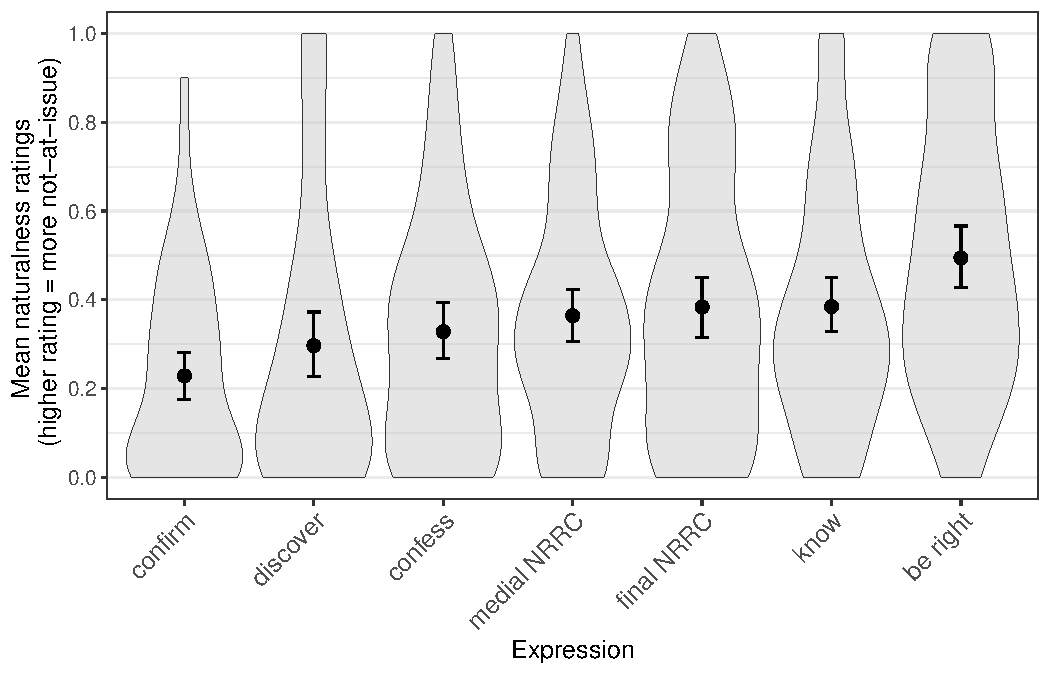
\includegraphics[width=.48\textwidth]{../../results/main/exp1/graphs/mean-ratings.pdf}
            \label{fig:qud}
        }
        \subfloat[`asking whether' ratings]{
            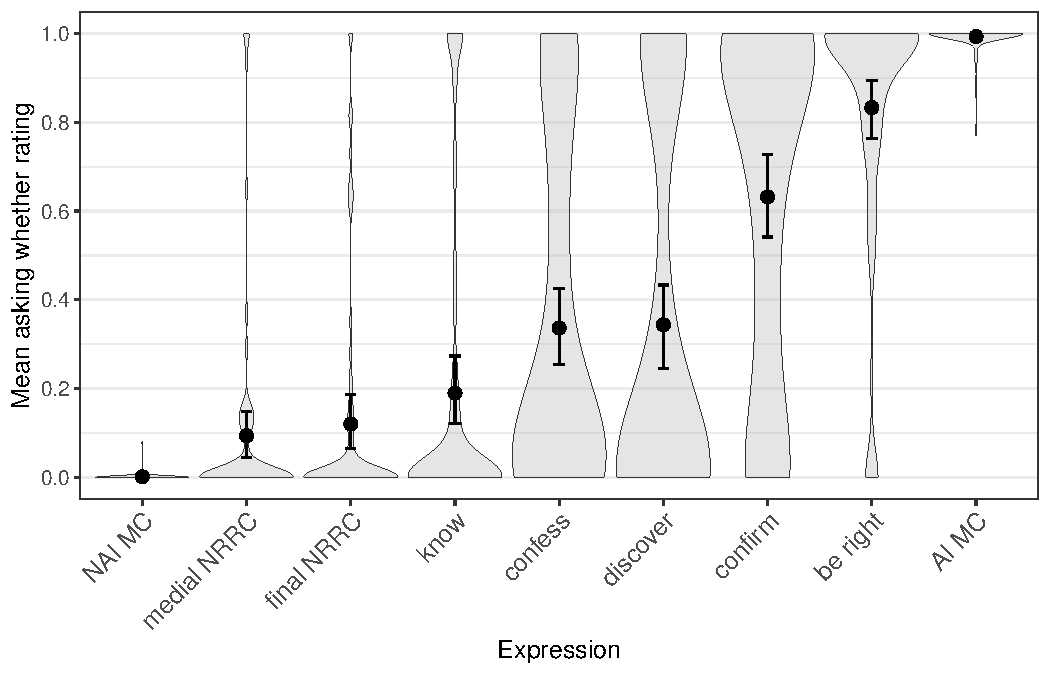
\includegraphics[width=.48\textwidth]{../../results/main/exp2/graphs/mean-ratings.pdf}
            \label{fig:AK}
        }\\
        \vspace{-\baselineskip}
        \subfloat[Naturalness ratings for the `direct dissent' diagnostic]{
            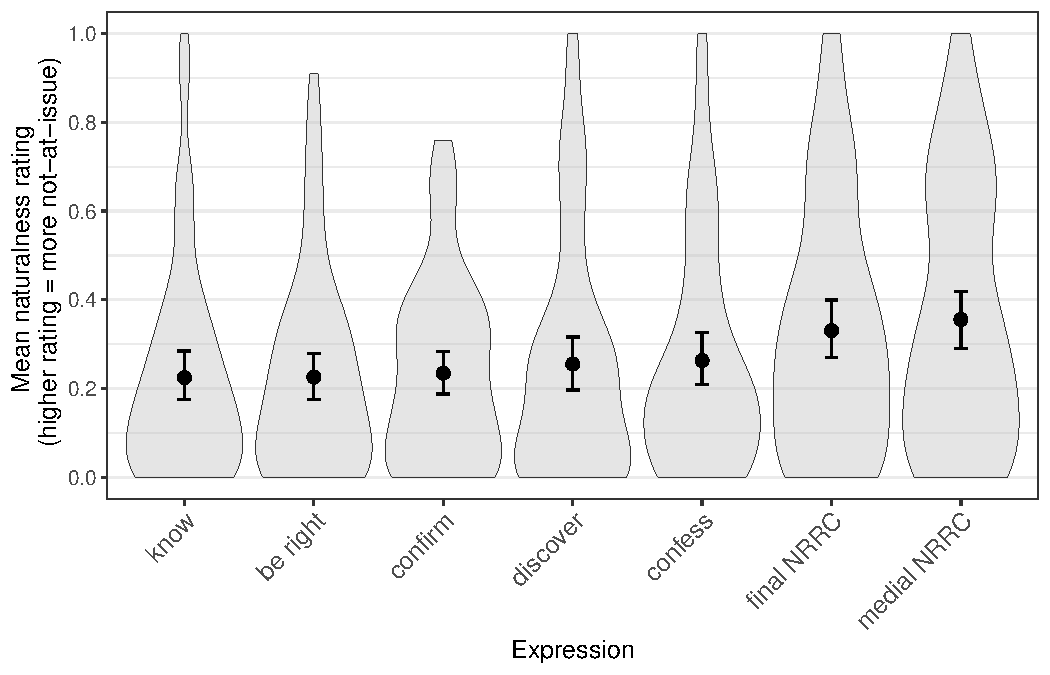
\includegraphics[width=.48\textwidth]{../../results/main/exp3/graphs/mean-ratings.pdf}
            \label{fig:dd}
        }
    \end{figure}

    \begin{figure}[ht]
    \vspace{-2\baselineskip}
      \caption{Proportion of ‘no’ choices by content for the `yes but' diagnostic. Error bars indicate 95\% bootstrapped confidence intervals. Gray dots indicate individual participant responses (either ‘no’ or one of the ‘yes’-responses, jittered vertically and horizontally for legibility).} \label{fig:yb}
      \vspace{-.5\baselineskip}
      \centering
      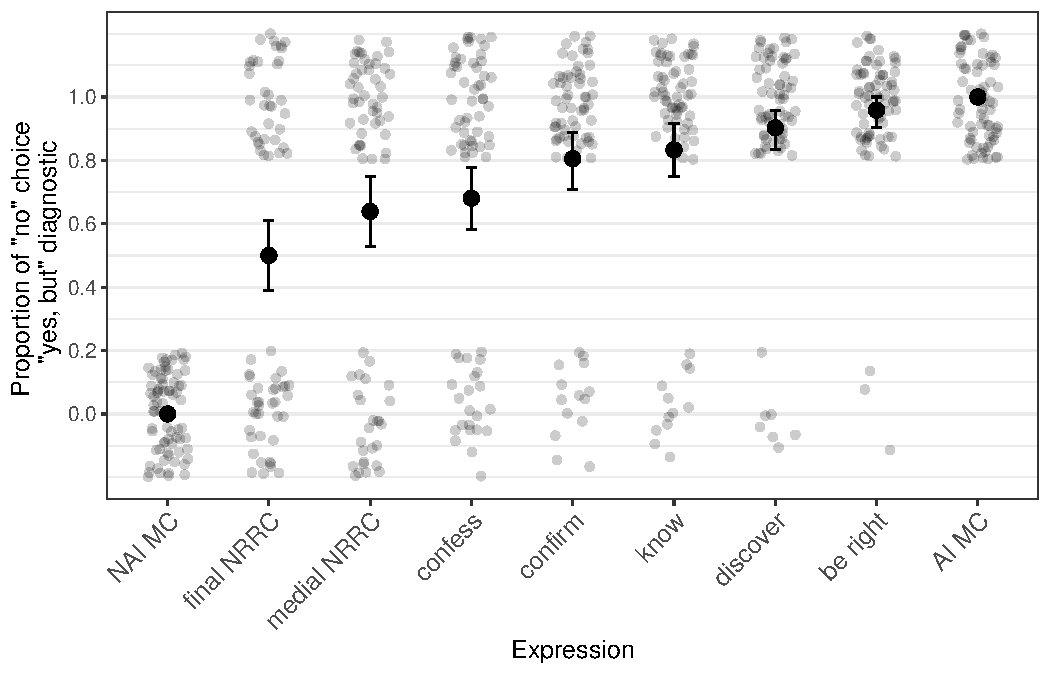
\includegraphics[width=.48\textwidth]{../../results/main/exp4/graphs/mean-ratings.pdf}
    \end{figure}

    Second, the content manipulation affects the ratings differently across the four diagnostics, sometimes in opposite directions. This results in a different order of predicates by response means between experiments.
    \begin{itemize}
      \item For instance, \emph{be right} ranks highest under the `asking whether' diagnostic (\Cref{fig:AK}), and the `yes, but' test (\Cref{fig:yb}), but ranks lowest under the QUD-diagnostic (\Cref{fig:qud}), and shows no clear effect in the direct dissent diagnostic (\Cref{fig:dd}).
    \end{itemize}
    

    \paragraph{Analysis.}
    \begin{itemize}
      \item Analysis similar to what we did in projection study? -- Interaction effects
      \item How about something similar to the rank-analysis that Yvonne Kilian did for comparing diagnostics?

    \end{itemize}


  \subsection{Discussion.}
    The differening results between diagnostics suggest that they are not interchangeable.

    \subsubsection{Sensitivity}

      \begin{itemize}
        \item Further, while the `asking whether' diagnostic, for contents embedded in questions, is sensitive enough to detect fine-grained differences between contents, the smaller range of response means for the other diagnostics could suggest the need for a more sensitive diagnostic for contents embedded in declarative assertions.

        \item We did not replicate the effect reported in \citealt{syrett_experimental_2015}, that sentence-final NRRCs receive higher at-issueness ratings than sentence-medial ones.

        \item  Additional comparison to \citealt{syrett_experimental_2015} (details omitted in the abstract) points to potential effects of the response task and the speech act of the utterance embedding the tested content.

      \end{itemize}

    \subsubsection{Order}

      \begin{itemize}
        \item In particular, the varying relative order of by-content means across diagnostics provide an initial argument that they target distinct properties of the content.
      \end{itemize}


\section{Conlusions and outlook}

  \subsection{Forward vs backward looking} % (fold)

    \citealt{koev_notions_2018}: Another notion of at-issueness: C-at-issueness, which is assumed to be a gerenalization of P-at-issueness;

    - right frontier constraint

    - some utterances, in subordinating relations do not move the QUD forward, see QUD stacks, Büring d-trees, and literature on relationship between QUD and discourse relations

    - other utterances, in coordinating relations, do move the QUD forward

    - that is why forward-looking and backward looking distinction is important 

    \begin{itemize}
      \item Q-AI ness + QUD diagnostic are about previous discourse
      \item P-AI ness and tonhauser's (\emph{issue} I-AI ness) are about the upcoming discourse
      \item can utterances shift the QUD? QUD-stack; adèle hernot-mortier?
      \item conditionals, sentence-medial vs sentence-final appositives
      \item co-ordination vs subordinating discourse relations and moving the discourse forward 
      \item possible confound: do the direct dissent diagnostic and the `yes, but' test P-at-issueness or anaphoric availability (\cite{snider_distinguishing_2018})
    \end{itemize}  
  
  % subsection forward_vs_backward_looking (end)

  \subsection{Questions vs assertions} % (fold)
      \begin{itemize}
        \item Q-AI ness and I-AIness are about question partitions
        \item P-AI ness is about assertive proposals
        \item is the speech-act distinction relevant? table model (and potentially some QUD implementations) suggest that this difference shouldnt matter
        \item possible counfound: commitment related to projection that we discussed in relation to the big study
      \end{itemize}
      
      \paragraph{Based on our data:} % (fold)
      
      \begin{itemize}
        \item the speech act seems to matter: the `asking whether' diagnostic, targeting questions...
      \end{itemize}

  % subsection questions_and_assertions (end)

  \subsection{Other diagnostics} % (fold)
    
  
  % subsection other_diagnostics (end)

  \begin{itemize}
    \item Other diagnostics (Horn on argumentation / because-clauses; evaluative adjectives)
  \end{itemize}


\pagebreak
\bibliographystyle{plainnat}
\bibliography{../at-issueness}

  

\end{document}